\subsection{Unlocking the Magic of Prescalers in Frequency Counting!}

\begin{tcolorbox}[colback=gray!10, colframe=black, title=E4A05]  
What is the purpose of using a prescaler with a frequency counter?  
\begin{enumerate}[label=\Alph*.]
    \item Amplify low-level signals for more accurate counting
    \item Multiply a higher frequency signal so a low-frequency counter can display the operating frequency
    \item Prevent oscillation in a low-frequency counter circuit
    \item \textbf{Reduce the signal frequency to within the counter's operating range}
\end{enumerate} \end{tcolorbox}

\subsubsection{Elaboration on Related Concepts}

In radio communication and electronics, a prescaler is a crucial component used with frequency counters to enable them to operate accurately within specific frequency ranges. Frequency counters are devices that measure the frequency of input signals. However, many frequency counters have a limited frequency range or can only accurately measure frequencies that fall within their operational limits.

Prescalers serve to address this limitation by reducing the frequency of the incoming signal. This reduction allows a frequency counter designed for lower frequency ranges to effectively measure higher frequency signals. The most common uses of prescalers are found in applications where signal frequencies exceed the counter's maximum input frequency.

\subsubsection{Understanding the Purpose of Prescalers}

1. \textbf{Operational Range}: Frequency counters have typical rate limits beyond which they may produce inaccurate readings. Prescalers ensure that the incoming signals are scaled down to a level that the counter can handle effectively.

2. \textbf{Common Types of Prescalers}: There are various types of prescalers, including divide-by-2, divide-by-4, to more complex programmable options that can divide by any integer value. By dividing the frequency of the input signal, they allow for a broader range of frequencies to be monitored accurately.

3. \textbf{Importance in Measurement}: Without prescalers, attempting to measure high-frequency signals could lead to non-linearities and erroneous data due to the limitations of the frequency counter's internal components.

In this particular question, option D, Reduce the signal frequency to within the counter's operating range, represents the principal function of a prescaler—ensuring that incoming signals are manageable for the frequency counting device.

\subsubsection{Example Calculation}
If a prescaler has a division factor of 10 and it receives a 100 MHz signal, the output frequency to the frequency counter will be:

\[
\text{Output Frequency} = \frac{\text{Input Frequency}}{\text{Division Factor}} = \frac{100 \, \text{MHz}}{10} = 10 \, \text{MHz}
\]

Thus, the frequency counter can measure this output frequency accurately within its operating range.

\subsubsection{Diagram}
To illustrate the concept visually, we can depict the signal input, the prescaler action, and the frequency counter. The following TikZ code can be used to create this diagram.

\begin{center}
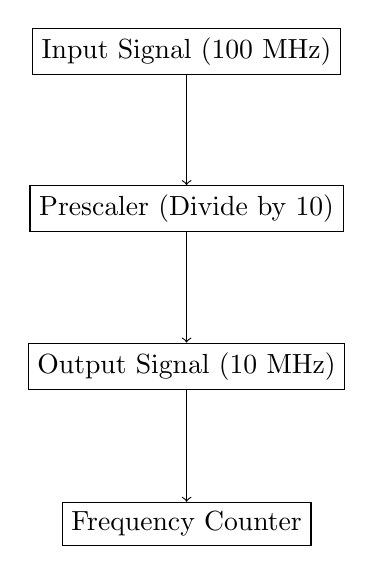
\begin{tikzpicture}[node distance=2cm]
    \node (input) [draw, rectangle] {Input Signal (100 MHz)};
    \node (prescaler) [draw, rectangle, below of=input] {Prescaler (Divide by 10)};
    \node (output) [draw, rectangle, below of=prescaler] {Output Signal (10 MHz)};
    \node (counter) [draw, rectangle, below of=output] {Frequency Counter};

    \draw[->] (input) -- (prescaler);
    \draw[->] (prescaler) -- (output);
    \draw[->] (output) -- (counter);
\end{tikzpicture}
\end{center}
